\documentclass[a4paper, 11pt, twoside]{article}

%\usepackage[ngerman]{babel}
\usepackage[english]{babel}
\usepackage[latin1]{inputenc}

\usepackage{graphicx,float}
%\usepackage{pifont}
\usepackage{type1cm}
\usepackage{amssymb, amsthm, amsmath}
\usepackage{listings}
\usepackage{pgf}
\usepackage{url}
\usepackage{hyperref}

\usepackage{makeidx}
\makeindex

\setlength{\parindent}{0em}
\setlength{\oddsidemargin}{0.0cm}
\setlength{\evensidemargin}{0.0cm}
\setlength{\textheight}{24.0cm}
\setlength{\topmargin}{-1.0cm}
\setlength{\footskip}{1.5cm}
\setlength{\textwidth}{15.5cm}

\renewcommand*\familydefault{\sfdefault}
\newcommand{\dd}{\mathrm{d}}
\newtheorem{problem}{Problem}[section]
\newtheorem{theorem}{Theorem}[section]
\newtheorem{remark}{Remark}[section]

\begin{document}
\pagestyle{empty}
\include{frontpage_hiflow_flow_tutorial}

%\newpage
%\null\newpage

\tableofcontents

\newpage
\pagestyle{plain}
\framebox[15.5cm]{\parbox[c][2.3cm]{14.5cm}{
{\fontsize{19}{19}\selectfont{} \bf{Using HiFlow$^3$ for solving the incompressible\\[0.5em] Navier-Stokes equations}
}}}
\vspace{0.5cm}
\section{Introduction}

HiFlow$^3$ is a multi-purpose finite element software providing powerful tools for efficient and accurate solution of a wide range of problems modeled by partial differential equations (PDEs). Based on object-oriented concepts and the full capabilities of C++ the HiFlow$^3$ project follows a modular and generic approach for building efficient parallel numerical solvers. It provides highly capable modules dealing with the mesh setup, finite element spaces, degrees of freedom, linear algebra routines, numerical solvers, and output data for visualization. Parallelism - as the basis for high performance simulations on modern computing systems - is introduced on two levels: coarse-grained parallelism by means of distributed grids and distributed data structures, and fine-grained parallelism by means of platform-optimized linear algebra back-ends.

\subsection{How to Use the Tutorial?}
You find the example code (flow\_tutorial.cc, flow\_tutorial.h) and a parameter file for the first numerical example (flow\_tutorial.xml) in the folder \verb'/hiflow/examples/flow'. The geometry data (*.inp, *.vtu) is stored in the folder \verb'/hiflow/examples/data'.

\subsubsection{Using HiFlow$^3$ as a Developer}\label{sectiondeveloper}
First build and compile HiFlow$^3$. Go to the directory \verb'/build/example/flow', where the binary \textbf{flow\_tutorial} is stored. Type \textbf{./flow\_tutorial}, to execute the program in sequential mode. To execute in parallel mode \index{program!executing in parallel} with four processes, type \textbf{mpirun -np 4 ./poisson\_tutorial}. In both cases, you need to make sure that the default parameterfile flow\_tutorial.xml is stored in the same directory as the binary, and that the geometry data specified in the parameter file is stored in \verb'/hiflow/examples/data'. Alternatively, you can specify the path of your own xml-file with the name of your xml-file (first) and the path of your geometry data (second) in the comment line, i.e. \textbf{./flow\_tutorial} \verb'/"path_to_parameterfile"/"name_of_parameterfile".xml' \verb'/"path_to_geometry_data"/'.

\section{Mathematical Setup}

\subsection{Problem}

We consider the simulation of a stationary laminar flow in a two-dimensional channel around a rectangular obstacle. 
\setlength{\unitlength}{1cm}
\begin{figure}[!h]
	\centering
		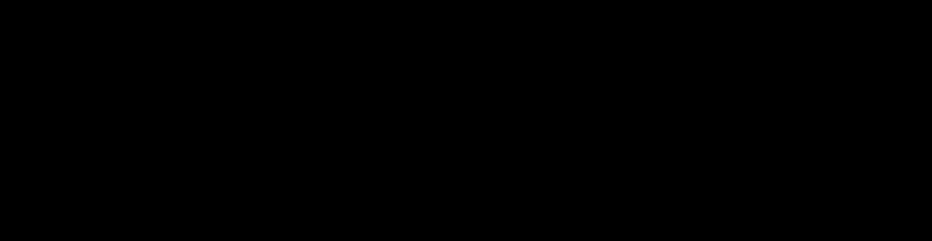
\includegraphics[width=1.1\textwidth]{fig/Zeichnung_Kanal_en.png}
		\begin{picture}(1,1)(-1.25,-1.2)
		\put(-8.2,1.6){\footnotesize{$u(x_1, x_2) =$}}
		\put(-8.2,1.1){\footnotesize{$g(x_1, x_2)$}}
		\put(1.1,3.7){\footnotesize{$u(x_1, x_2) = 0$}}
		\put(1.1,0.35){\footnotesize{$u(x_1, x_2) = 0$}}
		\end{picture}
\vspace{-0.75cm}
\caption{Flow channel in 2D with an obstacle.}
\label{channel}
\end{figure}
We assume the liquid to be an incompressible Newtonian fluid, and model the flow by the Navier-Stokes equations.\index{equation!Navier-Stokes}
To obtain the unique solution in 2D case the formulation of the problem is completed by setting appropriate
conditions on the boundary of the channel. We have to distinguish three different conditions, namely, (\ref{NR1}) the inflow condition at  $\Gamma_{\text{in}}$, (\ref{NR2}) the outflow at the end of the channel $\Gamma_{\text{out}}$
and (\ref{NR3}) the no-slip condition
at all remaining parts of the boundary $\Gamma_0$. Here, the outflow condition is chosen as a natural or
so-called do-nothing condition. We consider following boundary value problem for the unknown velocity field $u = (u_1(x_1, x_2), u_2(x_1,x_2))^T$ and the unknown pressure $p = p(x_1, x_2)$ of the velocity field:

\begin{align}
\label{eq:NS_strong1}\tag{1a}
-\nu \Delta u + (u \cdot \nabla ) u + \frac{1}{\rho} \nabla p &= 0, \quad \text{ in } \Omega,\\
\label{eq:NS_strong2}\tag{1b}
	 \nabla \cdot u &= 0, \quad \text{ in } \Omega,\\
 \label{NR1}\tag{1c}
u &= g, \quad \text{ on } \Gamma_{\text{in}},\\ 
\label{NR2}\tag{1d}
(- \mathcal{I} p + \nu \nabla u) \cdot n &= 0, \quad \text{ on } \Gamma_{\text{out}},\\
 \label{NR3}\tag{1e}
 	u &= 0, \quad \text{ on } \partial\Omega \backslash (\overline{\Gamma_{\text{in}} \cup \Gamma_{\text{out}}})=:\Gamma_0,  
 \end{align}   

where $\Omega$ is the domain specified in Fig \ref{channel}.
The viscosity\index{viscosity} $\nu = \nu(x_1, x_2)$ is a known material constant and the
density\index{density} $\rho = \rho(x_1, x_2)$ is also constant due to the incompressibility of the fluid. 
$ n = n(x, y)$ is the outer normal vector on $ \partial \Omega$ and $ \mathcal {I} \in \mathbb {R} ^ {2 \times 2} $ the unit matrix and $g:\Gamma_{\text{in}}\rightarrow \mathbb{R}$ is a given Dirichlet data. \\
In section \ref{section3D} we show some numerical results for the flow channel in three-dimensional case. We refer to  \cite{Turek96recentbenchmark} for detailed explanation of the 3D geometry.

\subsection{Solving the non-linear problem with Newton's method}\index{Newton's method}

The non-linear term $(u\cdot \nabla)u$ turns the Navier-Stokes equation\index{equation!Navier-Stokes}\index{equation!non-linear} (\ref{eq:NS_strong1}) into a non-linear equation. One possibility 
to solve a non-linear problem is using iterative Newton's method, which in general is a method to find the zero of a function $F$, i.e. 
\begin{align*}
F(\xi)=0,
\end{align*}
where $\xi$ represents the solution. The corresponding Newton-Iteration has the form:
\begin{align}
&\quad\xi^{k+1}:=\xi^k-\underbrace{(\nabla F(\xi^k))^{-1}F(\xi^k)}_{=:c^k}\ ,\qquad k=0,1,2,\ldots \nonumber\\
&\qquad \Longleftrightarrow \nonumber\\
&\begin{cases}
\nabla F(\xi^k)c^k=F(\xi^k) \\
\xi^{k+1}=\xi^k-c^k  \quad \textnormal{(update-step)} 
\end{cases},\label{Newtonstep}
\end{align}
where $c^k$ denotes the correction term and the start solution $\xi^0$ is given.  %\\
The term $\nabla F(\xi^k)c^k$ denotes the linearization,\index{linearization} which is the derivative of $F$ at the linearization point $\xi^k$ in the direction $c^k$. In our case $F$ is defined as:
\begin{align}
F(u^k,p^k):=\begin{pmatrix}F_1(u^k,p^k)\\ F_2(u^k,p^k)\end{pmatrix} = \begin{pmatrix}-\nu \Delta u^k + (u^k \cdot \nabla ) u^k + \frac{1}{\rho} \nabla p^k \\  \nabla \cdot u^k  \end{pmatrix}
\label{residual}
\end{align}

The derivation of the linearisation of the linear terms of (\ref{residual}) is trivial. Therefore it is only shown for the non-linear term $G(u):=(u\cdot \nabla)u$ (the index $k$ is omitted for simplicity):
\begin{align*}
\nabla_u G(u)\cdot c_u&=\underset{\varepsilon\rightarrow0}{\lim}\frac{1}{\varepsilon}(G(u+\varepsilon c_u)-G(u))\\
&=\underset{\varepsilon\rightarrow0}{\lim}\frac{1}{\varepsilon}\left[((u+\varepsilon c_u)\cdot \nabla)(u+\varepsilon c_u)-(u\cdot \nabla) u \right]\\
&=\underset{\varepsilon\rightarrow0}{\lim}\frac{1}{\varepsilon}\left[(u\cdot \nabla)(u+\varepsilon c_u)+(\varepsilon c_u \cdot \nabla)(u+\varepsilon c_u)-(u\cdot \nabla) u \right]\\
&=\underset{\varepsilon\rightarrow0}{\lim}\frac{1}{\varepsilon}\left[(u\cdot \nabla)u+(u\cdot \nabla)\varepsilon c_u+(\varepsilon c_u \cdot \nabla)u+(\varepsilon c_u\cdot \nabla)\varepsilon c_u-(u\cdot\nabla) u \right]\\
&=\underset{\varepsilon\rightarrow0}{\lim}\left[(u\cdot \nabla)c_u+(c_u\cdot \nabla)u+( c_u \cdot \nabla)\varepsilon c_u\right]\\
&=(u\cdot \nabla) c_u + (c_u\cdot \nabla)u  .
\end{align*}
 

The linearization of $F$ is then given by:
\begin{align*}
\nabla F(u,p)\cdot \begin{pmatrix}	c_u \\ c_p\end{pmatrix} = \begin{pmatrix}-\nu \Delta c_u + (u\cdot \nabla ) c_u +(c_u\cdot \nabla ) u+ \frac{1}{\rho} \nabla c_p \\ \nabla \cdot c_u \end{pmatrix}\, ,
\end{align*}
where the boundary conditions for $(c_u, c_p)^T$ are given by
\begin{equation*}
\begin{aligned}	
c_u &= 0 \quad \text{on} ~\Gamma_{\text{in}},\\
 (- \mathcal{I} c_p + \nu \nabla c_u) \cdot n &= 0 \quad \text{on} ~\Gamma_{\text{out}},\\ 	
 c_u &= 0 \quad \text{on} ~\Gamma_0\, .
\end{aligned}
\end{equation*}

\subsection{Weak Formulation}\index{weak formulation}
To solve a problem using finite element methods, a variational formulation of the problem must be given. 
It can be derived by multiplying the equation with some test functions, integrating over the domain, applying integration by parts and the Gauss theorem. 
Therefore the domain $\Omega$ has to be a Lipschitz domain \cite[p.89-96]{mclean}.

The solution space for the velocity $u$ is defined as 
\begin{align*}
 \mathcal{U}(\Omega) := \{ u\in (H^1(\Omega))^2: \ u|_{\Gamma_{\text{in}}} = g ,
\ u|_{\Gamma_0}= 0 \}.
\end{align*}

The space of test and trial functions has homogeneous Dirichlet boundaries. 
Therefore we have to find $\bar{u}= u+u_d$, where $u_d \in \mathcal{U}(\Omega)$ and
%The space $\mathcal{U}(\Omega)$ is suitable as the ansatz space, 
%because the Dirichlet conditions are fulfilled. But the test functions $\phi$ are zero at the Dirichlet boundaries. 
%Therefore we have to choose $\bar{u}= u+u_d$, where $u_d \in H^1$, which fulfill the right Dirichlet conditions. Thus it holds
\begin{align*}
u\in   V(\Omega) := \{ u\in (H^1(\Omega))^2 : \
u|_{\Gamma_0 \cup \Gamma_{\text{in}}}= 0\}.
\end{align*} 
  
In each Newton step (\ref{Newtonstep}) a problem of the following form has to be solved:
\begin{problem}
Find $c_u\in \mathcal{U}(\Omega)$ and $c_p\in L^2(\Omega)$ such that
\begin{equation} 
\begin{aligned}
  \int_{\Omega}\nu \nabla c_u : \nabla \phi + (\bar{u} \cdot \nabla) c_u \circ \phi + (c_u \cdot \nabla) \bar{u} \circ \phi
 %\\&
 - \frac{c_p}{\rho} (\nabla \circ \phi) \dd x &= \int_{\Omega} F_1(\bar{u},\bar{p}) \circ \phi \dd x ,\\ 
  \int_{\Omega} (\nabla \cdot c_u) \psi \ \dd x &= \int_{\Omega} F_2(\bar{u},\bar{p}) \circ \psi \dd x ,
 \end{aligned}\label{eq:NS_schwach} 
\end{equation}
for all test functions $\phi =(\phi_1,\phi_2)^T \in V(\Omega)$ and $\psi \in L^2(\Omega)$, where $(\bar{u},\bar{p})^T$ denotes the linearization point and is known (solution of the last Newton-Iteration step or start-solution). $\circ$ 
denotes the multiplication by components and $:$ the scalar product of two matrices 
($\nabla u : \nabla \phi = (\sum_{i} \frac{\partial u_i}{\partial x_j} \frac{\partial \phi_i}{\partial x_j})_j$), where $j$ denotes the index of the columns $(j=1,2)$ for the two components of the velocity.\\
\end{problem}

For the more general instationary case the following propositions about existence and uniqueness for the Navier-Stokes equations hold. For the theoretical statements we use the spaces 
\begin{align*}
V = \{ u\in (H^1_0(\Omega))^d : \int_{\Omega} (\nabla \cdot u)\psi = 0\quad \forall \psi \in L^2(\Omega)\}\ ,  \\
H = \{ u\in (L^2(\Omega))^d : \int_{\Omega} (\nabla \cdot u)\psi = 0\quad \forall \psi \in L^2(\Omega),\ u\cdot n = 0 \}\ ,
\end{align*}
which are solenoidal in weak sence and differ from the spaces defined before to solve the problem numerically. Using these solenoidal spaces, the equation for the pressure is fulfilled by definition and hence can be neglected.

Note also that the existence\index{solution!existence} and uniqueness\index{solution!uniqueness} depend on the space dimension \cite{sohr,temam}:
\begin{theorem}
Let $d \in \{2,3\}$. For the right hand side $g \in L^2(0,T;V)$ and the initial solution $u_0 \in H$ exists at least a weak solution.
\end{theorem}
\begin{theorem}
For the case $d=2$ the weak solution for the velocity $u$ is unique and even a strong solution.
\end{theorem}
\begin{theorem}
For the case $d=3$ exists at most a strong solution for the velocity $u$. 
\end{theorem}

Using the finite element method for the discretization, the linear variational formulation (\ref{eq:NS_schwach}) 
results in a stiffness matrix, which corresponds to $\nabla F(\xi^k)$ in the step (\ref{Newtonstep}) of Newton's method. 
During the discretization process the stiffness matrix and residual vector have to be assembled.\index{assembling!stiffness matrix} 

%\begin{figure}[!h]%
%	\centering
%		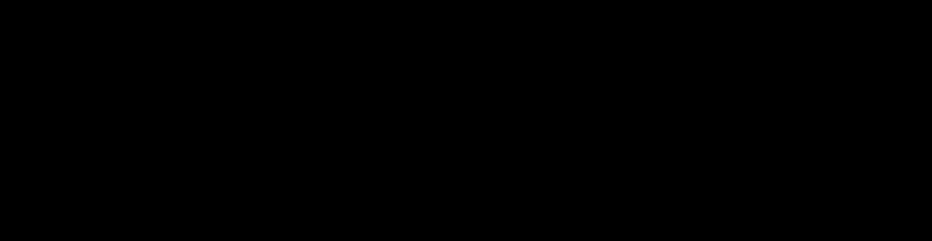
\includegraphics[width=0.9\textwidth]{fig/Zeichnung_Kanal_en.png}
%\caption{Flow channel in 2D.}
%\label{bild1}
%\end{figure}

\section{The Commented Program}

\subsection{Preliminaries}
HiFlow$^3$ is designed for high performance computing on massively parallel machines. 
So it applies the Message Passing Interface (MPI)\index{Message Passing Interface (MPI)}\index{MPI} library specification for message-passing, see sections \ref{main}, \ref{run}, \ref{read-mesh}. 
The flow tutorial needs following two input files:
\begin{itemize}
\item A parameter file: The parameter file is an xml-file, which contains all parameters needed to execute the program. It is read in by the program. Parameters for example defining the termination condition of the non-linear and linear solver are listed as well as parameters needed for the linear algebra. It is not necessary to recompile the program, when parameters in the xml-file are changed. By default the flow tutorial reads in the parameter file flow\_tutorial.xml, see section \ref{sectionparameter file}, which contains the parameters of the two-dimensional numerical example, see section \ref{section2D}.This file is stored in \verb'/hiflow/examples/flow/'. 
\item Geometry data\index{geometry data}: The file containing the geometry is specified in the parameter file. For the numerical results in two dimensions in section \ref{section2D} we choose dfg2d\_rect.inp. In section \ref{section3D} we choose dfg\_bench3d\_rect2.inp. You can find different meshes in the folder \newline \verb'/hiflow/examples/data' .
\end{itemize}

HiFlow$^3$ does not generate meshes for the domain $\Omega$.\index{domain geometry!generating} Meshes in *.inp and *.vtu format can be read in. It exists a function in \verb'/build/utils/' called 'inp2vtu' which converts *.inp format to *.vtu format. Type \textbf{/build/utils/inp2vtu 2 dfg2d\_rect.inp} to convert dfg2d\_rect.inp to dfg2d\_rect.vtu. Additionally a file dfg2d\_rect\_bdy.vtu is created which shows the body of the domain.\\
It is possible to extend the reader for other formats.
Furthermore it is possible to generate other geometries by using external programs (Mesh generators) or by hand. 
Both formats provide the possibility to mark cell or facets by material numbers.\\ 
%
To distinguish different boundary conditions on the boundary different material numbers are set. You can find different material numbers for some given geometry files in figure (\ref{materialnumbers}).
\begin{figure}[htb]
  \begin{tabular}{|l|l|l|l|l|l|l|l|}
  \hline
  File & \multicolumn{7}{|l|}{Material numbers} \\
  \hline
  & Inflow & Outflow & Top & Bottom & Obstacle & Front & Back \\
  \hline
  dfg2d\_rect.inp & 15 & 16 & 13 & 13 & 14 & - & - \\
  \hline
  channel\_2d\_uniform.inp & 10 & 12 & 13 & 11 & none & - & - \\
  \hline
  dfg\_bench3d\_cyl.inp & 10 & 12 & 11 & 11 & 13 & 11 & 11 \\
  \hline
  dfg\_bench3d\_rect2.inp & 10 & 12 & 11 & 11 & 13 & 30 & 20 \\
  \hline
  channel\_bench1.inp & 10 & 12 & 13 & 11 & 2/1(up/down) & 30 & 20 \\
  \hline
  \end{tabular}
\caption{Material numbers\index{material numbers} for different geometry files.}
\label{materialnumbers}
\end{figure}
The parameter file defines the meaning of the material number:
In the parameter file (flow\_tutorial.xml) you find the boundary parameters InflowMaterial and OutflowMaterial. 
In this case the variable InflowMaterial is set to 15 and the variable OutflowMaterial to 16. In the function prepare\_bc(), see section \ref{sec:prepare}, 
these parameters are read in, so that the program can distinguish the different parts of the boundary and 
set the correct boundary condition.\index{boundary condition!setting}\\

\subsection{Parameter File}\index{parameter file}\label{sectionparameter file}
The needed parameters are initialized in the paramter file flow\_tutorial.xml.
\begin{lstlisting}[language=C++, basicstyle={\footnotesize, \ttfamily}, keywordstyle=\color{blue}, numbers=none, tabsize=4]
<Param>
  <OutputPrefix>flow_tutorial</OutputPrefix>
  <Mesh>
    <Filename>dfg2d_rect.inp</Filename>
    <InitialRefLevel>0</InitialRefLevel>
  </Mesh>
  <LinearAlgebra>
    <NameMatrix>CoupledMatrix</NameMatrix>
    <NameVector>CoupledVector</NameVector>
    <Platform>CPU</Platform>
    <Implementation>Naive</Implementation>
    <MatrixFormat>CSR</MatrixFormat>
  </LinearAlgebra>
  <FlowModel>
    <Type>Channel</Type>
    <Density>1.0</Density>
    <Viscosity>1.0e-3</Viscosity>
    <InflowSpeed>0.3</InflowSpeed>
    <InflowHeight>0.41</InflowHeight>
    <InflowWidth>0.41</InflowWidth>
    <LidSpeed>0.3</LidSpeed>
  </FlowModel>
  <FiniteElements>
    <VelocityDegree>2</VelocityDegree>
    <PressureDegree>1</PressureDegree>
  </FiniteElements>
  <Instationary>
    <SolveInstationary>0</SolveInstationary>
    <Method>CrankNicolson</Method>
    <Timestep>0.1</Timestep>
    <Endtime>10.0</Endtime>
  </Instationary>
  <Boundary>
    <InflowMaterial>15</InflowMaterial>
    <OutflowMaterial>16</OutflowMaterial>
    <LidMaterial>12</LidMaterial>
  </Boundary>
  <NonlinearSolver>
    <Name>Newton</Name>
    <MaxIterations>100</MaxIterations>
    <AbsTolerance>1.e-8</AbsTolerance>
    <RelTolerance>1.e-8</RelTolerance>
    <DivTolerance>1.e6</DivTolerance>
  </NonlinearSolver>
  <LinearSolver>
    <Name>GMRES</Name>
    <Method>NoPreconditioning</Method>
    <MaxIterations>1000</MaxIterations>
    <AbsTolerance>1.e-10</AbsTolerance>
    <RelTolerance>1.e-10</RelTolerance>
    <DivTolerance>1.e6</DivTolerance>
    <SizeBasis>100</SizeBasis>
  </LinearSolver>
  <!--- WARNING: Pressure filter might not be suitable for the 
  	current formulation of the problem -->
  <UsePressureFilter>0</UsePressureFilter>
</Param>

\end{lstlisting}

\subsection{Main Function}\label{main}\index{MPI}
The main function starts the simulation of the flow problem (flow\_tutorial.cc).

\begin{lstlisting}[language=C++, basicstyle={\footnotesize, \ttfamily}, keywordstyle=\color{blue},  numbers=none, tabsize=4]
int main ( int argc, char** argv )
{
    MPI_Init ( &argc, &argv );

    // set default parameter file
    std::string param_filename ( PARAM_FILENAME );
    std::string path_mesh;
    // if set take parameter file specified on console
    if ( argc > 1 )
    {
        param_filename = std::string ( argv[1] );
    }
    // if set take mesh following path specified on console
    if ( argc > 2 )
    {
        path_mesh = std::string ( argv[2] );
    }
    try
    {
        FlowTutorial app ( param_filename, path_mesh );
        app.run ( );
    }
    catch ( std::exception& e )
    {
        std::cerr << "\nProgram ended with uncaught exception.\n";
        std::cerr << e.what ( ) << "\n";
        return -1;
    }
    MPI_Finalize ( );
    return 0;
}
\end{lstlisting}

\subsection{Member Functions}
Following member functions are components of the Navier-Stokes equation tutorial: 
\begin{itemize}
 \item run()
 \item read\_mesh()
 \item prepare()
 \item prepare\_bc()
 \item solve()
 \item EvalFunc(const LAD::VectorType\& u, LAD::VectorType* F)
 \item compute\_residual(const LAD::VectorType\& u, LAD::VectorType* F)
 \item compute\_stationary\_residual(const LAD::VectorType\& u, LAD::VectorType* F)
 \item EvalGrad(const LAD::VectorType\& u, LAD::MatrixType* DF)
 \item compute\_jacobian(const LAD::VectorType\& u, LAD::MatrixType* DF)
 \item compute\_stationary\_matrix(const LAD::VectorType\& u, LAD::MatrixType* DF)
 \item visualize()
\end{itemize}

\subsubsection{run()}\index{MPI}\label{run}
The member function run() calls the functions solve() and visualize() to solve the stationary flow problem and to generate the  data for the visualization.The function is defined in the class FlowTutorial (flow\_tutorial.cc).

\begin{lstlisting}[language=C++, basicstyle={\footnotesize, \ttfamily}, keywordstyle=\color{blue},  numbers=none, tabsize=4]
void FlowTutorial::run ( )
{
    simul_name_ = params_["OutputPrefix"].get<std::string>( );

    std::ofstream info_log ( ( simul_name_ + "_info_log" ).c_str ( ) );
    LogKeeper::get_log ( "info" ).set_target ( &info_log );
    std::ofstream debug_log ( ( simul_name_ + "_debug_log" ).c_str ( ) );
    LogKeeper::get_log ( "debug" ).set_target ( &debug_log );

    // output parameters for debugging
    LOG_INFO ( "parameters", params_ );

    flow_model_ = params_["FlowModel"]["Type"].get<std::string>( );

    if ( flow_model_ != std::string ( "Channel" ) &&
         flow_model_ != std::string ( "Cavity" ) )
    {
        throw UnexpectedParameterValue ( "FlowModel.Type", flow_model_ );
    }

    MPI_Comm_rank ( comm_, &rank_ );
    MPI_Comm_size ( comm_, &num_partitions_ );

    read_mesh ( );

    // The simulation has two modes: stationary and
    // instationary. Which one is used, depends on the parameter
    // Instationary.SolveInstationary. In stationary mode, solve()
    // is only called once, whereas in instationary mode, it is
    // called several times via the time-stepping method implemented in
    // run_time_loop() .
    solve_instationary_ =
            params_["Instationary"]["SolveInstationary"].get<bool>( );
    while ( !is_done_ )
    {
        prepare ( );
        if ( solve_instationary_ )
        {
            LOG_INFO ( "simulation", "Solving instationary problem" );
            run_time_loop ( );
        }
        else
        {
            LOG_INFO ( "simulation", "Solving stationary problem" );
            solve ( );
            visualize ( );
        }
        adapt ( );
    }
}
\end{lstlisting}

\subsubsection{read\_mesh()}\label{read-mesh}\index{MPI}
The member function read\_mesh() reads in the mesh. Depending if it was compiled with or without metis (\url{www.cs.umn.edu/~metis}), metis or the naive implementation is used for the partitioning of the mesh when executed in parallel  (flow\_tutorial.cc).

\begin{lstlisting}[language=C++, basicstyle={\footnotesize, \ttfamily}, keywordstyle=\color{blue},  numbers=none, tabsize=4]
void FlowTutorial::read_mesh ( )
{
    if ( rank ( ) == MASTER_RANK )
    {
        const std::string mesh_name =
                params_["Mesh"]["Filename"].get<std::string>( );
        std::string mesh_filename;
        if ( path_mesh.empty ( ) )
        {
            mesh_filename = std::string ( DATADIR ) + mesh_name;
        }
        else
        {
            mesh_filename = path_mesh + mesh_name;
        }

        master_mesh_ = read_mesh_from_file ( mesh_filename, DIMENSION, 
                                             DIMENSION, 0 );

        refinement_level_ = 0;
        const int initial_ref_lvl = params_["Mesh"]["InitialRefLevel"].
            get<int>( );

        for ( int r = 0; r < initial_ref_lvl; ++r )
        {
            master_mesh_ = master_mesh_->refine ( );
            ++refinement_level_;
        }
        LOG_INFO ( "mesh", "Initial refinement level = " << refinement_level_ );
    }

    MeshPtr local_mesh = partition_and_distribute ( master_mesh_, MASTER_RANK,
                                                    comm_ );
    assert ( local_mesh != 0 );
    SharedVertexTable shared_verts;
    mesh_ = compute_ghost_cells ( *local_mesh, comm_, shared_verts );

    std::ostringstream rank_str;
    rank_str << rank ( );

    PVtkWriter writer ( comm_ );
    std::string output_file = std::string ( "mesh_local.pvtu" );
    writer.add_all_attributes ( *mesh_, true );
    writer.write ( output_file.c_str ( ), *mesh_ );
}
\end{lstlisting}

\subsubsection{prepare()}\label{sec:prepare}
The member function prepare() reads in the needed parameters, initializes the linear algebra objects and calls the member function prepare\_bc() (flow\_tutorial.cc).

\begin{lstlisting}[language=C++, basicstyle={\footnotesize, \ttfamily}, keywordstyle=\color{blue},  numbers=none, tabsize=4]
void FlowTutorial::prepare ( )
{
    // prepare timestep
    ts_ = 0;
    dt_ = params_["Instationary"]["Timestep"].get<double>( );

    // Set the alpha coefficients correctly for the
    // Crank-Nicolson method.
    alpha1_ = 0.5 * dt_;
    alpha2_ = dt_;
    alpha3_ = 0.5 * dt_;

    // prepare problem parameters
    rho_ = params_["FlowModel"]["Density"].get<double>( );
    nu_ = params_["FlowModel"]["Viscosity"].get<double>( );

    if ( flow_model_ == std::string ( "Channel" ) )
    {
        Um_ = params_["FlowModel"]["InflowSpeed"].get<double>( );
        H_ = params_["FlowModel"]["InflowHeight"].get<double>( );
#if DIMENSION == 3
        W_ = params_["FlowModel"]["InflowWidth"].get<double>( );
#endif
    }
    else if ( flow_model_ == std::string ( "Cavity" ) )
    {
        Um_ = params_["FlowModel"]["LidSpeed"].get<double>( );
        std::cout << "Reynold's number = " << 1. / nu_ << "\n";
    }

    // prepare space
    std::vector< int > degrees ( DIMENSION + 1 );
    const int u_deg = params_["FiniteElements"]["VelocityDegree"].get<int>( );
    const int p_deg = params_["FiniteElements"]["PressureDegree"].get<int>( );
    for ( int c = 0; c < DIMENSION; ++c )
    {
        degrees.at ( c ) = u_deg;
    }
    degrees.at ( DIMENSION ) = p_deg;

    space_.Init ( degrees, *mesh_ );

    // pressure filter
    use_pressure_filter_ = params_["UsePressureFilter"].get<bool>( );

    // prepare linear algebra structures
    couplings_.Clear ( );
    couplings_.Init ( communicator ( ), space_.dof ( ) );

    // compute matrix graph

    std::vector < std::vector<bool> > coupling_vars;
    coupling_vars.resize ( DIMENSION + 1 );
    for ( int i = 0; i < DIMENSION; ++i )
    {
        for ( int j = 0; j < DIMENSION + 1; ++j )
        {
            coupling_vars[i].push_back ( true );
        }
    }
    for ( int i = 0; i < DIMENSION; ++i )
    {
        coupling_vars[DIMENSION].push_back ( true );
    }
    coupling_vars[DIMENSION].push_back ( false );

    SparsityStructure sparsity;
    global_asm_.compute_sparsity_structure ( space_, sparsity, &coupling_vars );

    couplings_.InitializeCouplings ( sparsity.off_diagonal_rows,
                                     sparsity.off_diagonal_cols );

    CoupledMatrixFactory<Scalar> CoupMaFact;
    matrix_ = CoupMaFact.Get (
            params_["LinearAlgebra"]["NameMatrix"].get<std::string>( ) )->
            params ( params_["LinearAlgebra"] );
    matrix_->Init ( communicator ( ), couplings_ );
    CoupledVectorFactory<Scalar> CoupVecFact;
    sol_ = CoupVecFact.Get (
            params_["LinearAlgebra"]["NameVector"].get<std::string>( ) )->
            params ( params_["LinearAlgebra"] );
    sol_->Init ( communicator ( ), couplings_ );
    prev_sol_ = CoupVecFact.Get (
            params_["LinearAlgebra"]["NameVector"].get<std::string>( ) )->
            params ( params_["LinearAlgebra"] );
    prev_sol_->Init ( communicator ( ), couplings_ );
    res_ = CoupVecFact.Get (
            params_["LinearAlgebra"]["NameVector"].get<std::string>( ) )->
            params ( params_["LinearAlgebra"] );
    res_->Init ( communicator ( ), couplings_ );

    matrix_->InitStructure ( vec2ptr ( sparsity.diagonal_rows ),
                             vec2ptr ( sparsity.diagonal_cols ),
                             sparsity.diagonal_rows.size ( ),
                             vec2ptr ( sparsity.off_diagonal_rows ),
                             vec2ptr ( sparsity.off_diagonal_cols ),
                             sparsity.off_diagonal_rows.size ( ) );
    matrix_->Zeros ( );

    sol_->InitStructure ( );
    sol_->Zeros ( );

    prev_sol_->InitStructure ( );
    prev_sol_->Zeros ( );

    rhs_ = CoupVecFact.Get (
            params_["LinearAlgebra"]["NameVector"].get<std::string>( ) )->
            params ( params_["LinearAlgebra"] );
    rhs_->Init ( communicator ( ), couplings_ );
    rhs_->InitStructure ( );
    rhs_->Zeros ( );

    res_->InitStructure ( );
    res_->Zeros ( );

    // prepare dirichlet BC
    prepare_bc ( );
}
\end{lstlisting}

\subsubsection{prepare\_bc()}
The member function prepare\_bc() sets up the Dirichlet boundary\index{boundary condition!modelling} values (flow\_tutorial.cc).

\begin{lstlisting}[language=C++, basicstyle={\footnotesize, \ttfamily}, keywordstyle=\color{blue},  numbers=none, tabsize=4]
void FlowTutorial::prepare_bc ( )
{
    dirichlet_dofs_.clear ( );
    dirichlet_values_.clear ( );

    if ( flow_model_ == std::string ( "Channel" ) )
    {
        const int inflow_bdy = params_["Boundary"]["InflowMaterial"].
            get<int>( );
        const int outflow_bdy = params_["Boundary"]["OutflowMaterial"].
            get<int>( );
#if DIMENSION == 2
        ChannelFlowBC2d bc[2] = { ChannelFlowBC2d ( 0, H_, Um_, 
                                                    inflow_bdy, outflow_bdy ),
                                  ChannelFlowBC2d ( 1, H_, Um_, 
                                                    inflow_bdy, outflow_bdy ) };
#endif

#if DIMENSION == 3
        ChannelFlowBC3d bc[3] = { ChannelFlowBC3d ( 0, W_, H_, Um_, 
                                                    inflow_bdy, outflow_bdy ),
                                  ChannelFlowBC3d ( 1, W_, H_, Um_, 
                                                    inflow_bdy, outflow_bdy ),
                                  ChannelFlowBC3d ( 2, W_, H_, Um_, 
                                                    inflow_bdy, outflow_bdy ) };
#endif
        for ( int var = 0; var < DIMENSION; ++var )
        {
            compute_dirichlet_dofs_and_values ( bc[var], space_, var,
                                                dirichlet_dofs_, 
                                                dirichlet_values_ );
        }
    }
    else if ( flow_model_ == std::string ( "Cavity" ) )
    {
        const int lid_bdy = params_["Boundary"]["LidMaterial"].get<int>( );

        LidCavityBC bc[2] = { LidCavityBC ( 0, Um_, lid_bdy ),
                             LidCavityBC ( 1, Um_, lid_bdy ) };

        for ( int var = 0; var < DIMENSION; ++var )
        {
            compute_dirichlet_dofs_and_values ( bc[var], space_, var,
                                                dirichlet_dofs_, 
                                                dirichlet_values_ );
        }
    }
    else
    {
        assert ( false );
    }

    // apply BC to initial solution
    if ( !dirichlet_dofs_.empty ( ) )
    {
        // correct solution with dirichlet BC
        sol_->SetValues ( vec2ptr ( dirichlet_dofs_ ), 
                          dirichlet_dofs_.size ( ),
                          vec2ptr ( dirichlet_values_ ) );
    }
}
\end{lstlisting}


The boundary conditions are defined in the class ChannelFlowBC (flow\_tutorial.h).

\begin{lstlisting}[language=C++, basicstyle={\footnotesize, \ttfamily}, keywordstyle=\color{blue},  numbers=none, tabsize=4]
struct ChannelFlowBC2d
{
    // Parameters:
    // var - variable
    // H - channel height
    // Um - maximum inflow
    // inflow_bdy - material number of inflow boundary
    // outflow_bdy - material number of outflow boundary

    ChannelFlowBC2d ( int var, double H, double Um, int inflow_bdy, int outflow_bdy )
    : var_ ( var ), H_ ( H ), Um_ ( Um ), inflow_bdy_ ( inflow_bdy ),
    outflow_bdy_ ( outflow_bdy )
    {
        assert ( var_ == 0 || var_ == 1 );
    }

    std::vector<double> evaluate ( const Entity& face,
                                   const std::vector<Coord>& coords_on_face ) const
    {
        std::vector<double> values;

        const int material_num = face.get_material_number ( );

        const bool outflow = ( material_num == outflow_bdy_ );
        const bool inflow = ( material_num == inflow_bdy_ );

        // Dirichlet boundary conditions. Check whether
        // the face lies on an inflow boundary, and if so set
        // u_x = 4*Um * y * (1-y) / H^2 and u_y = 0. Otherwise, set u_x = u_y = 0 .

        if ( !outflow )
        {
            values.resize ( coords_on_face.size ( ) );

            // loop over points on the face
            for ( int i = 0; i < static_cast < int > ( coords_on_face.size ( ) ); 
                  ++i )
            {
                // evaluate dirichlet function at each point
                const Coord& pt = coords_on_face[i];

                if ( inflow )
                {
                    if ( var_ == 0 )
                    { // x-component
                        values[i] = 4. * Um_ * pt[1] * ( H_ - pt[1] ) / 
                            ( H_ * H_ );
                    }
                    else if ( var_ == 1 )
                    { // y-component
                        values[i] = 0.;
                    }
                    else
                    {
                        assert ( false );
                    }
                }
                else
                {
                    // not inflow: u = 0
                    values[i] = 0.;
                }
            }
        }
        return values;
    }

    const int var_;
    const double H_;
    const double Um_;
    const int inflow_bdy_, outflow_bdy_;
};
\end{lstlisting}

\subsubsection{solve()}\index{solver!non-linear}
The member function solve() reads in some parameters and solves the non-linear flow problem at the current time step using the Newton method (flow\_tutorial.cc).

\begin{lstlisting}[language=C++, basicstyle={\footnotesize, \ttfamily}, keywordstyle=\color{blue},  numbers=none, tabsize=4]
void FlowTutorial::solve ( )
{
    // setup linear solver
    LinearSolver<LAD>* linsolver_;
    LinearSolverFactory<LAD> LinSolFact;
    linsolver_ = LinSolFact.Get (
            params_["LinearSolver"]["Name"].get<std::string>( ) )->
            params ( params_["LinearSolver"] );
    linsolver_->SetupOperator ( *matrix_ );

    // setup nonlinear solver parameters
    NonlinearSolverFactory<LAD> NLSFact;
    nls_ = NLSFact.Get ( 
            params_["NonlinearSolver"]["Name"].get<std::string>( ) )->
            params ( res_, matrix_, params_["NonlinearSolver"] );

    // we use our own initial solution -- this needs to be indicated
    // to the Newton-solver
    if ( params_["NonlinearSolver"]["Name"].get<std::string>( ) == "Newton" )
        ( ( Newton<LAD>* )nls_ )->InitParameter ( Newton<LAD>::NewtonInitialSolutionOwn );

    nls_->SetOperator ( *this );
    nls_->SetLinearSolver ( *linsolver_ );

    NonlinearSolverState state = nls_->Solve ( *rhs_, sol_ );

    std::cout << "Nonlinear solver ended with state " << state
            << " and residual norm " << nls_->GetResidual ( )
            << " after " << nls_->iter ( ) << " iterations\n";

    LOG_INFO ( "Nonlinear solver residual", nls_->GetResidual ( ) );
    LOG_INFO ( "Nonlinear solver steps", nls_->iter ( ) );

    delete nls_;
    delete linsolver_;
}
\end{lstlisting}

\subsubsection{EvalFunc(const LAD::VectorType\& u, LAD::VectorType* F)}
The member function EvalFunc(const LAD::VectorType\& u, LAD::VectorType* F) evaluates the function at a given point u and is called in Solve(const VectorType\& rhs, VectorType* x) (see newton.cc). u is a vector given in and the evaluated function is returned.

\begin{lstlisting}[language=C++, basicstyle={\footnotesize, \ttfamily}, keywordstyle=\color{blue},  numbers=none, tabsize=4]
void FlowTutorial::EvalFunc ( const LAD::VectorType& u, LAD::VectorType* F )
{
    // compute the residual vector
    compute_residual ( u, F );
}
\end{lstlisting}

\subsubsection{compute\_residual(const LAD::VectorType\& u, LAD::VectorType* F)}\index{residual}
The member function compute\_residual(const LAD::VectorType\& u, LAD::VectorType* F) computes the residual for the Newton-method (flow\_tutorial.cc).

\begin{lstlisting}[language=C++, basicstyle={\footnotesize, \ttfamily}, keywordstyle=\color{blue},  numbers=none, tabsize=4]
void FlowTutorial::compute_residual ( const LAD::VectorType& u,
                                      LAD::VectorType* F )
{
    if ( solve_instationary_ )
    {
        compute_instationary_residual ( u, F );
    }
    else
    {
        compute_stationary_residual ( u, F );
    }

    // correct BC -- set Dirichlet dofs to 0
    if ( !dirichlet_dofs_.empty ( ) )
    {
        std::vector<LAD::DataType> zeros ( dirichlet_dofs_.size ( ), 0. );
        F->SetValues ( vec2ptr ( dirichlet_dofs_ ), dirichlet_dofs_.size ( ),
                       vec2ptr ( zeros ) );
    }
}
\end{lstlisting}

\subsubsection{compute\_stationary\_residual(const LAD::VectorType\& u, LAD::VectorType* F)}
The member function compute\_stationary\_residual(const LAD::VectorType\& u, LAD::VectorType* F) computes the residual for the stationary case (flow\_tutorial.cc).

\begin{lstlisting}[language=C++, basicstyle={\footnotesize, \ttfamily}, keywordstyle=\color{blue}, numbers=none, tabsize=4]
void FlowTutorial::compute_stationary_matrix ( const LAD::VectorType& u,
                                               LAD::MatrixType* DF )
{
    StationaryFlowAssembler local_asm ( u, nu_, rho_ );
    global_asm_.assemble_matrix ( space_, local_asm, *DF );
}

\end{lstlisting}

The operator for the assembling of the stationary residual is implemented in the class StationaryFlowAssembler (flow\_tutorial.h).

\begin{lstlisting}[language=C++, basicstyle={\footnotesize, \ttfamily}, keywordstyle=\color{blue}, numbers=none, tabsize=4]
    void operator() ( const Element<double>& element, 
                      const Quadrature<double>& quadrature,
                      LocalVector& lv )
    {
        AssemblyAssistant<DIMENSION, double>::initialize_for_element ( element, 
                                                                  quadrature );

        // recompute previous solution values
        for ( int v = 0; v < DIMENSION; ++v )
        {
            prev_vel_[v].clear ( );
            grad_prev_vel_[v].clear ( );
            evaluate_fe_function ( solution_, v, prev_vel_[v] );
            evaluate_fe_function_gradients ( solution_, v, grad_prev_vel_[v] );
        }
        pressure_k_.clear ( );
        evaluate_fe_function ( solution_, DIMENSION, pressure_k_ );

        const int num_q = num_quadrature_points ( );

        // loop over quadrature points
        for ( int q = 0; q < num_q; ++q )
        {
            const double wq = w ( q );
            const double dJ = std::abs ( detJ ( q ) );

            // get previous solution in vector form
            Vec<DIMENSION, double> vel_k;
            for ( int var = 0; var < DIMENSION; ++var )
            {
                vel_k[var] = prev_vel_[var][q];
            }

            // l1(v) = \nu * \int( \grad{u_k} : \grad{v} )
            for ( int v_var = 0; v_var < DIMENSION; ++v_var )
            {
                for ( int i = 0; i < num_dofs ( v_var ); ++i )
                {
                    lv[dof_index ( i, v_var )] += wq * ( nu_ * 
                            dot ( grad_phi ( i, q, v_var ), 
                            grad_prev_vel_[v_var][q] ) )
                            * dJ;
                }
            }

            // l2(v) = \int(u_k*\grad{u_k}*v)
            for ( int v_var = 0; v_var < DIMENSION; ++v_var )
            {
                for ( int i = 0; i < num_dofs ( v_var ); ++i )
                {
                    lv[dof_index ( i, v_var )] +=
                            wq * ( dot ( grad_prev_vel_[v_var][q], vel_k ) * 
                            phi ( i, q, v_var ) ) * dJ;
                }
            }

            // l3(v) = -1/rho*\int(p_k*div(v))
            for ( int v_var = 0; v_var < DIMENSION; ++v_var )
            {
                for ( int i = 0; i < num_dofs ( v_var ); ++i )
                {
                    lv[dof_index ( i, v_var )] +=
                            -wq * ( inv_rho_ * pressure_k_[q] * 
                            grad_phi ( i, q, v_var )[v_var] ) * dJ;
                }
            }

            // l4(q) = \int(q * div(u_k))
            const int q_var = DIMENSION;
            double div_u_k = 0.;
            for ( int d = 0; d < DIMENSION; ++d )
            {
                div_u_k += grad_prev_vel_[d][q][d];
            }

            for ( int i = 0; i < num_dofs ( q_var ); ++i )
            {
                lv[dof_index ( i, q_var )] +=
                        wq * ( inv_rho_ * div_u_k * phi ( i, q, q_var ) ) * dJ;
            }
        }
    }
\end{lstlisting}

\subsubsection{EvalGrad(const LAD::VectorType\& u, LAD::MatrixType* DF)}
The member function EvalGrad(const LAD::VectorType\& u, LAD::MatrixType* DF) computes the gradient at a given point u and is called in Solve(const VectorType\& rhs, VectorType* x) (see newton.cc). The vector u is given in and the gradient at u is returned.

\begin{lstlisting}[language=C++, basicstyle={\footnotesize, \ttfamily}, keywordstyle=\color{blue},  numbers=none, tabsize=4]
void FlowTutorial::EvalGrad ( const LAD::VectorType& u, LAD::MatrixType* DF )
{
    // assemble the matrix for the linearized system
    compute_jacobian ( u, DF );
}
\end{lstlisting}

\subsubsection{compute\_jacobian(const LAD::VectorType\& u, LAD::MatrixType* DF)}\index{Jacobian}
The member function compute\_jacobian(const LAD::VectorType\& u, LAD::MatrixType* DF) computes the Jacobian matrix for the Newton method (flow\_tutorial.cc).

\begin{lstlisting}[language=C++, basicstyle={\footnotesize, \ttfamily}, keywordstyle=\color{blue},  numbers=none, tabsize=4]
void FlowTutorial::compute_jacobian ( const LAD::VectorType& u,
                                      LAD::MatrixType* DF )
{
    if ( solve_instationary_ )
    {
        compute_instationary_matrix ( u, DF );
    }
    else
    {
        compute_stationary_matrix ( u, DF );
    }

    // correct BC -- set Dirichlet rows to identity
    if ( !dirichlet_dofs_.empty ( ) )
    {
        DF->diagonalize_rows ( vec2ptr ( dirichlet_dofs_ ), 
                               dirichlet_dofs_.size ( ), 1. );
    }
}
\end{lstlisting}

\subsubsection{compute\_stationary\_matrix(const LAD::VectorType\& u, LAD::MatrixType* DF)}
The member function compute\_stationary\_matrix(const LAD::VectorType\& u, LAD::MatrixType* DF) computes the Jacobian matrix for the stationary case (flow\_tutorial.cc).

\begin{lstlisting}[language=C++, basicstyle={\footnotesize, \ttfamily}, keywordstyle=\color{blue}, numbers=none, tabsize=4]
void FlowTutorial::compute_stationary_matrix ( const LAD::VectorType& u,
                                               LAD::MatrixType* DF )
{
    StationaryFlowAssembler local_asm ( u, nu_, rho_ );
    global_asm_.assemble_matrix ( space_, local_asm, *DF );
}
\end{lstlisting}

The operator for the assembling of the stationary matrix\index{assembling!stationary matrix} is implemented in the class StationaryFlowAssembler (flow\_tutorial.h).

\begin{lstlisting}[language=C++, basicstyle={\footnotesize, \ttfamily}, keywordstyle=\color{blue},  numbers=none, tabsize=4]
void operator() ( const Element<double>& element, 
                  const Quadrature<double>& quadrature,
                  LocalMatrix& lm )
    {
        AssemblyAssistant<DIMENSION, double>::initialize_for_element ( element,
                                                                  quadrature );

        // recompute previous solution values
        for ( int v = 0; v < DIMENSION; ++v )
        {
            prev_vel_[v].clear ( );
            grad_prev_vel_[v].clear ( );
            evaluate_fe_function ( solution_, v, prev_vel_[v] );
            evaluate_fe_function_gradients ( solution_, v, grad_prev_vel_[v] );
        }

        const int num_q = num_quadrature_points ( );

        // loop q
        for ( int q = 0; q < num_q; ++q )
        {
            const double wq = w ( q );
            const double dJ = std::abs ( detJ ( q ) );

            // get previous solution in vector form
            Vec<DIMENSION, double> vel_k;
            for ( int var = 0; var < DIMENSION; ++var )
            {
                vel_k[var] = prev_vel_[var][q];
            }

            // assemble a1(u,v) = \int {\grad(u) : \grad(v)}
            for ( int u_var = 0; u_var < DIMENSION; ++u_var )
            {
                for ( int i = 0; i < num_dofs ( u_var ); ++i )
                {
                    for ( int j = 0; j < num_dofs ( u_var ); ++j )
                    {
                        lm ( dof_index ( i, u_var ), dof_index ( j, u_var ) ) += 
                                 wq * ( nu_ *  dot ( grad_phi ( j, q, u_var ), 
                                 grad_phi ( i, q, u_var ) ) ) * dJ;
                    }
                }
            }

            // assemble a2(u,v) = \int { (vel_k*\grad{u})*v }
            for ( int u_var = 0; u_var < DIMENSION; ++u_var )
            {
                for ( int i = 0; i < num_dofs ( u_var ); ++i )
                {
                    for ( int j = 0; j < num_dofs ( u_var ); ++j )
                    {
                        lm ( dof_index ( i, u_var ), dof_index ( j, u_var ) ) +=
                                wq * ( dot ( vel_k, grad_phi ( j, q, u_var ) ) * 
                                phi ( i, q, u_var ) ) * dJ;
                    }
                }
            }

            // assemble a3(u,v) = \int { (u\grad{u_k}*v }
            for ( int test_var = 0; test_var < DIMENSION; ++test_var )
            {
                for ( int trial_var = 0; trial_var < DIMENSION; ++trial_var )
                {
                    for ( int i = 0; i < num_dofs ( test_var ); ++i )
                    {
                        for ( int j = 0; j < num_dofs ( trial_var ); ++j )
                        {
                            lm ( dof_index ( i, test_var ), dof_index(j, trial_var)) +=
                                    wq * ( grad_prev_vel_[test_var][q][trial_var] *
                                    phi ( j, q, trial_var ) *
                                    phi ( i, q, test_var ) ) * dJ;
                        }
                    }
                }
            }

            // assemble b(p, v) = - \int{p div{v}}
            const int p_var = DIMENSION;
            for ( int v_var = 0; v_var < DIMENSION; ++v_var )
            {
                for ( int i = 0; i < num_dofs ( v_var ); ++i )
                {
                    for ( int j = 0; j < num_dofs ( p_var ); ++j )
                    {
                        lm ( dof_index ( i, v_var ), dof_index ( j, p_var ) ) +=
                                -wq * ( inv_rho_ * phi ( j, q, p_var ) *
                                grad_phi ( i, q, v_var )[v_var] ) * dJ;
                    }
                }
            }

            // assemble bT(u, q) = \int{q div(u)}
            const int q_var = DIMENSION;
            for ( int u_var = 0; u_var < DIMENSION; ++u_var )
            {
                for ( int i = 0; i < num_dofs ( q_var ); ++i )
                {
                    for ( int j = 0; j < num_dofs ( u_var ); ++j )
                    {
                        lm ( dof_index ( i, q_var ), dof_index ( j, u_var ) ) +=
                                wq * ( inv_rho_ * phi ( i, q, q_var ) *
                                grad_phi ( j, q, u_var )[u_var] ) * dJ;
                    }
                }
            }
        }
    }
\end{lstlisting}

\subsubsection{visualize()}\label{sec:visualize}
The member function visualize() writes data for visualization\index{visualization} of the current solution (flow\_tutorial.cc).

\begin{lstlisting}[language=C++, basicstyle={\footnotesize, \ttfamily}, keywordstyle=\color{blue},  numbers=none, tabsize=4]
void FlowTutorial::visualize ( )
{

    int num_intervals = 2;
    ParallelCellVisualization<double> visu ( space_, num_intervals, comm_, 
                                             MASTER_RANK );

    std::stringstream input;

    input << simul_name_ << "_solution";

    if ( solve_instationary_ )
    {
        if ( ts_ < 10 )
            input << "000" << ts_;
        else if ( ts_ < 100 )
            input << "00" << ts_;
        else if ( ts_ < 1000 )
            input << "0" << ts_;
        else
            input << "" << ts_;
    }
    else
    {
        input << "_stationary";
    }

    std::vector<double> remote_index ( mesh_->num_entities ( mesh_->tdim ( ) ), 
                                       0 );
    std::vector<double> sub_domain ( mesh_->num_entities ( mesh_->tdim ( ) ), 
                                     0 );
    std::vector<double> material_number ( mesh_->num_entities ( mesh_->tdim ( ) ), 
                                        0 );

    for ( mesh::EntityIterator it = mesh_->begin ( mesh_->tdim ( ) );
          it != mesh_->end ( mesh_->tdim ( ) );
          ++it )
    {
        int temp1, temp2;
        mesh_->get_attribute_value ( "_remote_index_", mesh_->tdim ( ),
                                     it->index ( ),
                                     &temp1 );
        mesh_->get_attribute_value ( "_sub_domain_", mesh_->tdim ( ),
                                     it->index ( ),
                                     &temp2 );
        material_number.at ( it->index ( ) ) = 
             mesh_->get_material_number ( mesh_->tdim ( ), it->index ( ) );
        remote_index.at ( it->index ( ) ) = temp1;
        sub_domain.at ( it->index ( ) ) = temp2;
    }

    // Create visualization from post-processing vector.
    sol_->UpdateCouplings ( );
    visu.visualize ( EvalFeFunction<LAD>( space_, *( sol_ ), 0 ), "u" );
#if DIMENSION >= 2
    visu.visualize ( EvalFeFunction<LAD>( space_, *( sol_ ), 1 ), "v" );
#endif
#if DIMENION == 3
    visu.visualize ( EvalFeFunction<LAD>( space_, *( sol_ ), 2 ), "w" );
#endif
    visu.visualize ( EvalFeFunction<LAD>( space_, *( sol_ ), DIMENSION ), "p" );

    visu.visualize_cell_data ( material_number, "Material Id" );
    visu.visualize_cell_data ( remote_index, "_remote_index_" );
    visu.visualize_cell_data ( sub_domain, "_sub_domain_" );
    visu.write ( input.str ( ) );
}

\end{lstlisting}

\section{Program Output}
HiFlow$^3$ can be executed in a parallel or sequential mode which influence the generated output data. Note that the log files can be viewed by any editor.
\subsection{Parallel Mode}\index{parallel mode}
Executing the program in parallel, for example with four processes by \textbf{mpirun -np 4 ./flow\_tutorial}  \index{program!executing in parallel} 
generates following output data. 
\begin{itemize}
\item Mesh/geometry data:
\begin{itemize}
\item \textbf{mesh\_local.pvtu} Global mesh (parallel vtk-format). It combines the local meshes of sequential vtk-format owned by the different processes to the global mesh.
\item \textbf{mesh\_local\_X.vtu} local mesh owned by process X for X=0, 1, 2 and 3 (vtk-format).
\end{itemize}
\item Solution data. Since it is only possible to visualize data of polynomial degree 1 (Q1 on quads in 2 dimensions), 
only the data corresponding to the degrees of freedom of a Q1-element are written out. 
It means the information of the degrees of freedom of higher order is lost due to the fact that it cannot be visualized using the vtk-format.
\begin{itemize}
\item \textbf{flow\_tutorial\_solution\_stationary.pvtu} Solution of the velocity field and the pressure variable (parallel vtk-format). It combines the local solutions owned by the different processes to a global solution.
\item \textbf{flow\_tutorial\_solution\_stationary\_X.vtu} Local solution of the velocity field and the pressure variable of the degrees of freedoms which belong to cells owned by process X, for X=0, 1, 2 and 3 (vtk-format).
\end{itemize}
\item Log files:
\begin{itemize}
\item \textbf{flow\_tutorial\_debug\_log} Log file listing errors helping to simplify the debugging process. This file is empty if the program runs without errors.
\item \textbf{flow\_tutorial\_info\_log} Log file listing parameters and some helpful informations to control 
      the program as for example information about the residual of the linear and non-linear solver used.
\end{itemize}
\end{itemize}

\subsection{Sequential Mode}\index{sequential mode}
Exequting the program sequentially by \textbf{./flow\_tutorial} following output data is generated.\index{program!executing sequentially} 
\begin{itemize}
\item Mesh/geometry data:
\begin{itemize}
\item \textbf{mesh\_local.pvtu} Global mesh (parallel vtk-format). 
\item \textbf{mesh\_local\_0.vtu} Global mesh owned by process 0 (vtk-format) containing the mesh information.
\end{itemize}
\item Solution data. Since it is only possible to visualize data of polynomial degree 1 (Q1 on quads in 2 dimensions), only the data corresponding to the degrees of freedom of a Q1-element are written out. It means the information of the degrees of freedom of higher order are lost due to the fact that this information cannot be visualized using the vtk-format.
\begin{itemize}
\item \textbf{flow\_tutorial\_solution\_stationary.vtu} Solution of the velocity field and the pressure variable (vtk-format). 
\end{itemize}
\item Log files:
\begin{itemize}
\item \textbf{flow\_tutorial\_debug\_log} is a list of errors helping to simplify the debugging process. This file keeps empty if the program runs without errors.
\item \textbf{flow\_tutorial\_info\_log} is a list of parameters and some helpful informations to control the program as for example information 
                                         about the residual of the linear and non-linear solver used.
\end{itemize}
\end{itemize}

\subsection{Visualizing the Solution}\index{visualization}
HiFlow$^3$ only generates output data, see section \ref{sec:visualize}, but does not visualize. The mesh/geometry data as well as the solution data can be visualized 
by any external program which can handle the vtk data format as e.g. the program paraview \cite{Paraview}.\index{paraview} 


\section{Numerical Examples}

\subsection{Two-Dimensional Example}\label{section2D}
We choose a parabolic inflow condition namely, $g (x, y)= (4 U_m \frac {y (H-y)}{H^2},  0)^\top$ with $U_m = 0.3 ms^{-1}$, $H=0.41m$. 
This gives a stationary solution similar to a Poiseuille flow\index{Poiseuille flow}\footnote{In fluid dynamics, the Poiseuille equation is a physical 
law that gives the pressure drop in a fluid flowing through a long cylindrical pipe. The assumptions of the equation are that the flow is 
laminar viscous and incompressible and the flow is through a constant circular cross-section that is substantially longer than its diameter.}.


\begin{figure}[h!]
	\centering
		\includegraphics[width=1.1\textwidth]{fig/mesh_flow_tutorial_on_4_processes_trans.png}
\caption{Global 2D mesh of channel with obstacle partitioned over 4 processes.}
\label{mesh}
\end{figure}

\begin{figure}[h!]
	\centering
		\includegraphics[width=1.1\textwidth]{fig/u_velocity_with_mesh_flow_tutorial_trans.png}
\caption{Solution for the $u_1$-component(horizontal) of the velocity field together with the mesh.}
\label{sol_u1}
\end{figure}

\begin{figure}[h!]
	\centering
		\includegraphics[width=1.1\textwidth]{fig/v_velocity_flow_tutorial_trans.png}
\caption{Solution for the $u_2$-component(vertical) of the velocity field.}
\label{sol_u2}
\end{figure}

\begin{figure}[h!]
	\centering
		\includegraphics[width=1.1\textwidth]{fig/p_pressure_flow_tutorial_trans.png}
\caption{Solution for the pressure variable $p$.}
\label{sol_p}
\end{figure}

Fig. \ref{mesh} shows the discrete mesh and how it is distributed over four processes by metis (\url{www.cs.umn.edu/~metis}). Each color refers to on process.
The other three fig. \ref{sol_u1}, \ref{sol_u2}, \ref{sol_p} show the solution of the two velocity components $u_1$, $u_2$ and the pressure variable $p$ respectively for this example. 

\subsection{Three-Dimensional Example}\label{section3D}
In this example, we choose as inflow condition $g(x,y,z) = (16 U_m y z\frac{(H-y)(H-z)}{H^4}, 0, 0)^T$ (with the notation as in \cite{Turek96recentbenchmark}). We set $U_m = 0.3 ms^{-1}$ and $H=0.41m$ in the parameter file. As geometry data we choose the flow channel around a cylinder with square cross-section named dfg\_bench3d\_rect2.inp. Do not forget to adapt the material numbers, see table \ref{materialnumbers}, when changing your geometry data. Fig. \ref{mesh_3D}-\ref{pressure_3D} show the mesh, the solution for this example illustrated by vectors and the
pressure. 

\begin{remark}
To execute this example, you have to change the variable \verb'DIM' in the header file flow\_tutorial.h and afterwards compile the example again before executing.
\end{remark}

\begin{figure}[h!]
	\centering
		\includegraphics[width=1.1\textwidth]{fig/FlowtutGitter2trans.png}
\caption{The figure shows the mesh used for the simulation. It is a channel with a cylinder with square cross-section as obstacle.}
\label{mesh_3D}
\end{figure}

\begin{figure}[h!]
	\centering
		\includegraphics[width=1.1\textwidth]{fig/channel_benchmark_trans.png}
\caption{The figure shows the velocity vector field $u_h \in H_h(\Omega)$ of the simulation. The bigger the arrows, the higher the velocity.}
\label{sol_3D}
\end{figure}

\begin{figure}[h!]
	\centering
		\includegraphics[width=1.1\textwidth]{fig/FlowtutDrucktrans.png}
\caption{The figure shows the solution for the pressure.}
\label{pressure_3D}
\end{figure}

\newpage
\appendix
\bibliography{tutorials_bib}
\bibliographystyle{plain}

\printindex

\end{document}
